\chapter{Future Work}
\label{futureWork}

\section{Deficiencies in The Oronyminator}
\label{section:directImprovementsToMisheardMeOronymParseTree}

In some cases, our expected, UNISYN-derived phrase-frequency metric did not accurately line up with the observed transcription frequencies from our user studies.  We believe that there are several possible reasons for this.  

\subsection{Frequency Validity}
\label{subsection:frequencyValidity}
Our frequency source data from UNISYN ended up being less than statisfactory, due to several factors, deliniated below. 

\subsubsection{Corpus Composition deficiencies}
\label{futureWork:frequency:CorpusCompositionDeficiencies}

The lack of quality phonemic frequency data is a known defeciency in our source dictionary, UNISYN. According to the authors of the UNISYN lexicon documentation:
\begin{quote}
It should be noted that the frequency field, as it was obtained from simple word lists, is \emph{not particularly reliable} (emphasis mine).\cite{fitt_documentation_2000}  
\end{quote}
The UNISYN frequency count is based upon a large but not exhaustive corpus of text.  It has some particularly glaring deficiencies in the medical arena.  We find this frustrating, because knowledge about common medical mondegreens could be used to prevent mistakes in patient's treatment plans\cite{medicalMondegreensWhenIUseAWord}. Also, it meant that the word ``colitis'' wasn't in our dictionary, and we therefore couldn't use the example ``the girl with colitis goes by''/``the girl with kaleidescope eyes''. 


\subsubsection{Homograph Differentiation}
\label{futureWork:frequency:HomographDifferentiation}


Additionally, our source frequency data cannot and does not distinguish between words that may be homographs (that is, words that sound different but are spelled the same). This makes our program improperly weight some phrases over others. 

For example, take the words for the animals ``bucks'' and ``does''.  ``Bucks'' has a frequency of 1133, and ``does'' has a frequency of 508386.  For comparison, ``deer'' has a frequency of 1896.  You can see the relative scale of these in figure ~\ref{fig:DoesBucksDeerBubbleGraph}.  It seems highly unlikely that the male and female labels for a species would be as or more common than the actual name of the species, given that we don't see this for sheep (sheep at 13572 , ewe at 186 ,and  ram at 681) or horses (horse at 27559 , mare at 1055 , and stallion at 644 ).  What is much more likely is that ``bucks'' is getting extra hits through its meaning as a slang synonym for dollars (dollars at 8927), and ``does'' is getting most of its frequency count for the 3rd person present tense of the verb ``to do''.  That seems very likely, given that the frequency for the singular ``doe'' is only 1077. 

\begin{figure}
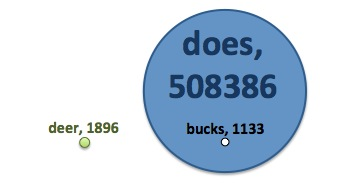
\includegraphics{DoesBucksDeerBubbleGraph.jpg}
\captionfonts
\caption[Bubble Chart comparison of Frequency for deer, does, and bucks]{Bubble Chart comparison of Frequency for deer, does, and bucks }
\label{fig:DoesBucksDeerBubbleGraph}
\end{figure}

Future work on our project would benefit from using a dictionary with some way of distinguishing homographs when counting frequency.


\subsubsection{Frequency Dictionary Tallying Methods}
\label{futureWork:frequency:freqDictTallyMethods}


In the future, we'd also like to use word frequency values from a dictionary that takes a larger, more-diverse dataset into its frequency count, such as the frequency lists from the Corpus of Contemporary American English\cite{freeFreqList}.  The COCA corpus is entirely focused on word frequency, and as such, does not contain any phonetic data.  However, it contains several different ways of determining frequency of words that overcome some of the shortcomings we ran into trying to compare the semantically-identical words `a' and `an'.  `A' is found much for frequently than `an', but both are just as common.  In the UNISYN dictionary, we only have contextless frequency counts.  In the COCA frequency dictionary, they keep two types of counts: one for how many times the word has been found total, and one for how many documents the word has been found in.  This way, even though `a' is found almost seven times as often than `a' overall, we know that they're equally-familiar words, because they are both found in approximately 160k corpus entries\cite{davies_word_2011}.

As a proof of concept, we created a sunburst diagram for ``an ice cold hour'' using COCA by-document frequency values (shown in figure ~\ref{fig:futureWork:COCAsunburst}), to compare it against the sunburst diagram created using UNISYN frequency values(shown in figure ~\ref{fig:futureWork:UNISYNsunburst}).  The COCA-based sunburst, while still inaccurate, at least has a ratio of phrases beginning with ``a'' to ``an'' that is closer to the actual observed ratio (which can be seen back in figure ~\ref{fig:results:aNiceColdHourObserved}).



\begin{figure}
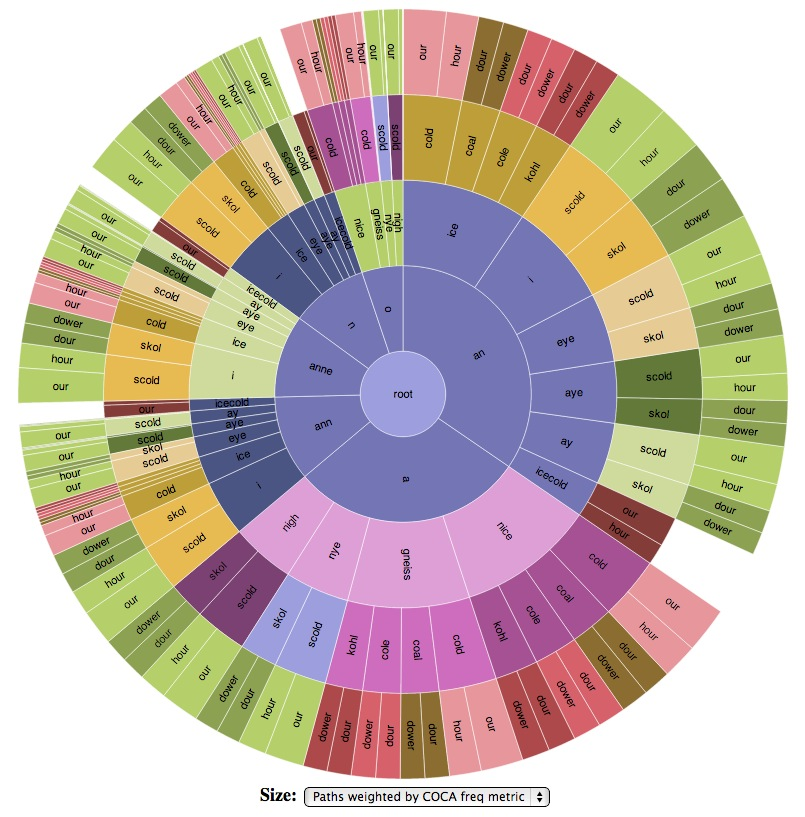
\includegraphics[width=\textwidth]{aNiceColdHour_COCA_FreqMetric.jpg}
\captionfonts
\caption[Sunburst diagram for ``an ice cold hour'' using COCA by-document freq metric]{Sunburst diagram for ``an ice cold hour'' using COCA by-document freq metric }
\label{fig:futureWork:COCAsunburst}
\end{figure}

\begin{figure}
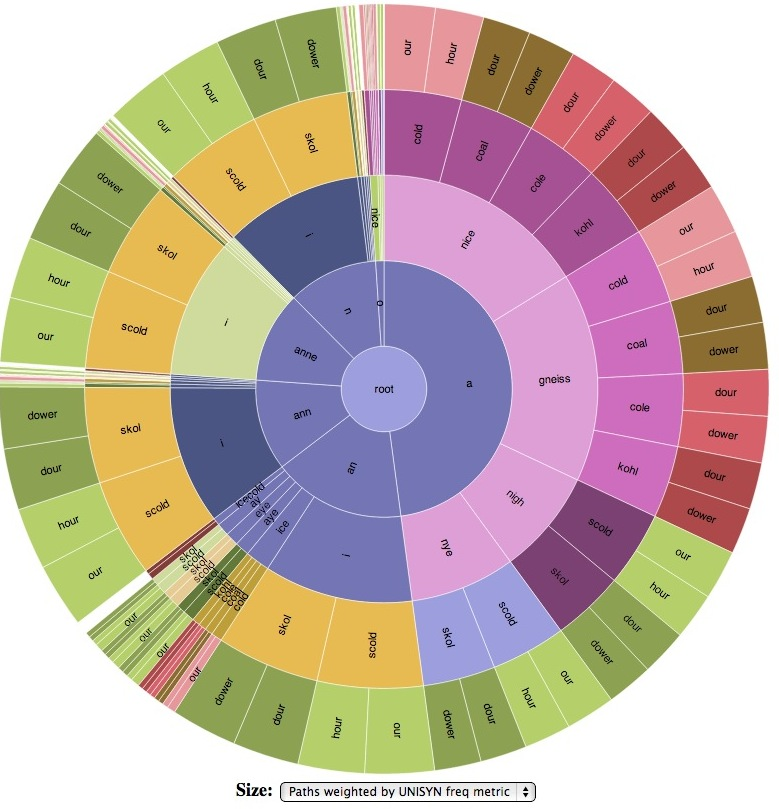
\includegraphics[width=\textwidth]{aNiceColdHour_UNISYN_FreqMetric.jpg}
\captionfonts
\caption[Sunburst diagram for ``an ice cold hour'' using UNISYN freq metric]{Sunburst diagram for ``an ice cold hour'' using UNISYN freq metric }
\label{fig:futureWork:UNISYNsunburst}
\end{figure}

%%%Insert here: statistics! Grab and adapt from 5.2.3 or something like that...


A statistical analysisof the observed dataset frequencies versus a COCA-derived frequency dataset, using a one-proportion z test, further proves that the COCA frequency values are a better match for the observed data than the UNISYN-derived frequencies.  Again using the top two observed transcriptions as our sample population, we take a look at the phrases \phraseOne and \phraseTwo.  The phrase \phraseOne has a calculated COCA freq metric of \cocaFreqForPhraseOne, and had \USATranscriptionsOfPhraseOne actual transcriptions observed among people living in the United States. The \phraseTwo has a calculated COCA freq metric of \cocaFreqForPhraseTwo, and had \USATranscriptionsOfPhraseTwo actual transcriptions observed among people living in the United States. Therefore, the expected population is \cocaCombinedFreq, and the observed population is \USACombinedTranscriptions.  

Given those population, the expected population proportion for \phraseOne would be \cocaFreqForPhraseOne  $\div$ \cocaCombinedFreq, or \expectedProportionOfPhraseOneOccurancesCOCA.  

In our user study, we found that \USATranscriptionsOfPhraseOne people transcribed \phraseOne, and \USATranscriptionsOfPhraseTwo people transcribed \phraseTwo, for a ratio of 0.65 to 1, where \phraseOne accounts for 39.56\% ( p = \observedProportionOfPhraseOneOccurances ) of the combined count. 

Given the observed population proportion of \observedProportionOfPhraseOneOccurances and the expected population proportion \expectedProportionOfPhraseOneOccurancesCOCA, we did a one-proportion z test with an $\alpha$ of \alphaSigFigs.  The z value returned was \COCAzVal, meaning that the observed population proportion was \COCAzVal standard deviations away from the expected population proportion.  When we used this z value to compute a p value, we were left with a pvalue of \pvalueCOCA, which is greater than our $\alpha$ of \alphaSigFigs. Therefore, there is approximately a 0.01\% chance that the observed data could match the COCA predictions, but it's still not incredibly likely. It's significantly more likely than the UNISYN predictions being correct, however.



\subsection{Higher-order frequency data}
\label{subsection:HigherOrderFrequencyData}

Right now, our program only takes into account the frequency of standalone words, without taking their context into consideration.  In the future, we'd like to integrate n-grams into our program. N-grams are a probabilistic model of predicting the next item that will follow in a sequence, based upon frequencies of how often those N items occur in sequence in a corpus of text\cite{ngramSiteFreeLists}.  A word-level 4-gram, for example, would be a series of four words. Here are some 4-gram phrases, along with counts of how often they occur, from the Google Ngram corpus:
\begin{quote}
serve as the informational 41 \\
serve as the infrastructure 500 \\
serve as the initial 5331\\
serve as the initiating 125\\
serve as the initiation 63\\
serve as the initiator 81\\
serve as the injector 56\\
serve as the inlet 41\\
serve as the inner 87\\
serve as the input 1323\\
\end{quote} \cite{allOurNgramsAreBelongToYou}

To give an example of what that might look like, we looked up historical n-gram occurence percentage of n-grams contained in oronyms of our main test phrase ``an ice cold hour''.  As seen in figure ~\ref{fig:futureWork:ThreeGram}, comparing the 3-grams ``a nice cold'' and ``an ice cold'' results in a fairly even split, though the latter phrase is slightly more likely to occur in modern-day settings. When we look at the 2-grams of that 3-gram, we see more interesting trends. In figure ~\ref{fig:futureWork:TwoGramAnice}, we see that ``a nice'' is consistently more frequently found in text than ``an ice'' is. However, when we compare the 2-grams ``ice cold'' and ``nice cold'', as we do in figure ~\ref{fig:futureWork:TwoGramIceCold}, we see that the phrase ``ice cold'' is leaps and bounds more likely to be encountered in everyday language.

\begin{figure}
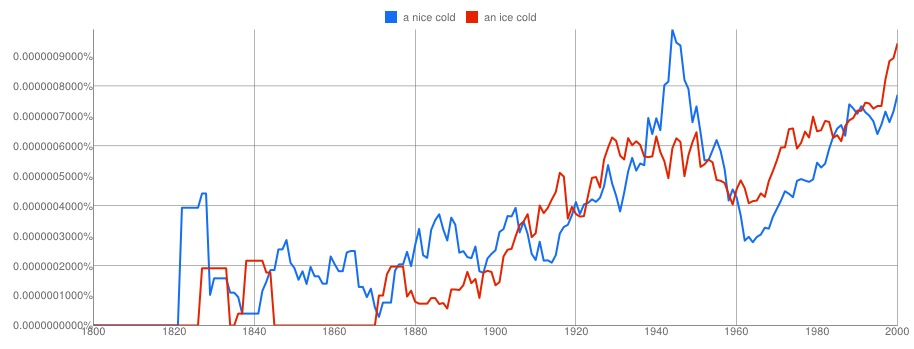
\includegraphics[width=\textwidth]{googleNgram_aNiceColdVSanIceCold.jpg}
\captionfonts
\caption[Historical N-gram data comparing the three-grams ``a nice cold'' and ``an ice cold'']{Historical N-gram data comparing the three-grams ``a nice cold'' and ``an ice cold''}
\label{fig:futureWork:ThreeGram}
\end{figure}


\begin{figure}
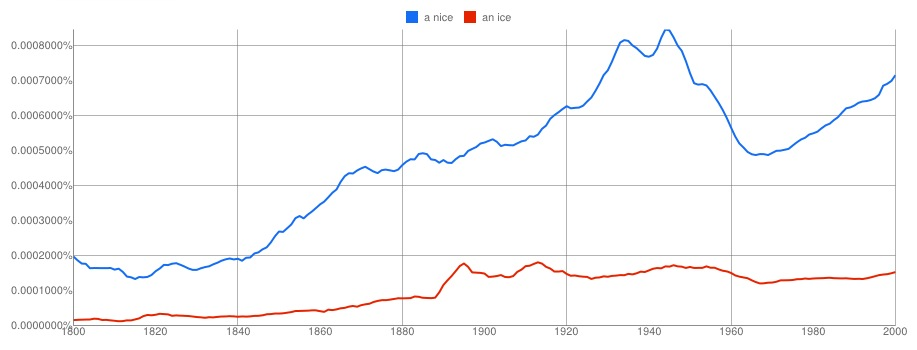
\includegraphics[width=\textwidth]{googleNgram_aNiceVSanIce.jpg}
\captionfonts
\caption[Historical N-gram data comparing the two-grams ``a nice'' and ``an ice'']{Historical N-gram data comparing the two-grams ``a nice'' and ``an ice''}
\label{fig:futureWork:TwoGramAnice}
\end{figure}

\begin{figure}
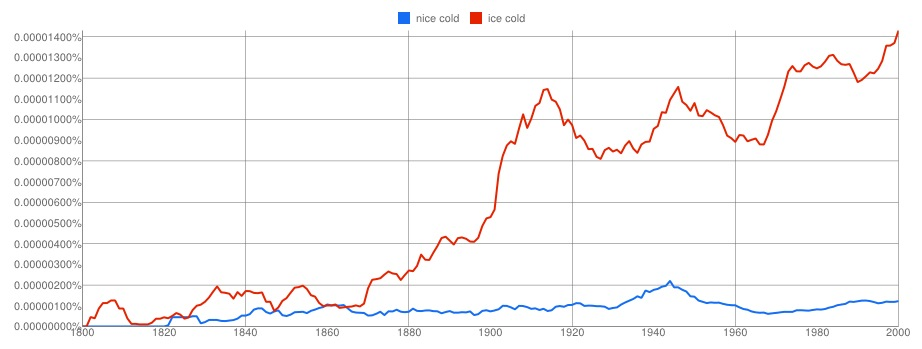
\includegraphics[width=\textwidth]{googleNgram_iceColdVSniceCold.jpg}
\captionfonts
\caption[Historical N-gram data comparing the two-grams ``nice cold'' and ``ice cold'']{Historical N-gram data comparing the two-grams ``nice cold'' and ``ice cold''}
\label{fig:futureWork:TwoGramIceCold}
\end{figure}


Though we are happy with our findings, we believe that we could create even better likelihood metrics with the integration of several different orders of n-grams, and would suggest this for future work.  However, if the final purpose of the oronyminator ends up being in the song lyric domain, everyday-usage syntactical predictability may not be particularly relevant, due to the differences in vocabulary and grammar found in song lyrics versus regular prose.


\section{Phoneme swapping}
\label{section:phonemeSwapping}

Often when speaking, humans substitute easier-to-say phones for more time-intensive phones.  One of the main ways that this substitution occurs is through voiced/voiceless pairs.  To “voice” a phone means to cause the vocal chords to vibrate.  “Voiced” phones are singable, whereas “voiceless” phones are not.  “Voiceless” phones are like a hiss, and simply direct streams of escaping air.  Most consonant phonemes are part of a voice/voiceless pair, such as `t' and `d' (The word ``pretty", when spoken quickly, often uses a `d' sound instead of a `t' sound, because the phoneme for `d' is easier to say). Phones are paired when the only differences between their pronuciation is the voicing, aka, when their manner of articulation (i.e. their manner of directing air during the sound), mouth end position, and mouth start position are the same (To view all phones in the SAMPA alphabet, along with enough information to determine whether they are pairs, see table ~\ref{sampaTable}). In our project, we came across an example of phoneme swapping in the ``cold''/``gold'' transcriptions, which we went over in figure ~\ref{fig:results:transcriptionCountPerRecordingANiceGoldHour} and section ~\ref{results:transcriptionCountPerRecording:a_nice_gold_hour}. For future work, we suggest looking into phoneme swap pairings, and integrating the findings into the existing algorithm. 


\section{Melody Matcher master project}
\label{melodyMatcherMasterProject}
MisheardMe Oronyminator is a part of the greater Melody Matcher suite. Melody Matcher is a semi-automated music composition support program. It analyzes English lyrics along with a melody, and alerts the composer of the locations in the song where the lyrics are not deterministically understandable. Basically, it's grammar- and spell-check for songs. 

\vspace{14pt}
Melody Matcher aims to replicate the human ability to identify lyrics in a song that are easily misheard. 
\vspace{14pt}

\subsection{Target Audience and Goals}
This program is to be used as a compositional aid by anyone who wants to write songs and make them sound good, technically. It should allow the song writer to focus on more subjective criteria of what makes a song ``good'', because it will make the structural rules of lyric composition immediately apparent.

Our hope for this project is that it will be useful to burgeoning songwriters, who have the creative spark to make wonderfully poetic lyrics, but lack the ``ear'' to match their lyrics successfully to music. It should be particularly helpful to songwriters who place a high emphasis on understandability of lyrics (such as parody song writers, or lyricists for musical theater).

Additionally, Melody Matcher will be useful for songwriters for whom English is a second language. While they may be a master lyricist in their native language, writing lyrics in English can be a particular challenge, since so much of lyric-writing is dependent upon knowing the cadence of the language you're writing lyrics in, and since English has no easily-discernible rules for emphasis placement in words.



While MisheardMe Oronyminator only takes into account phonetics and frequencies, Melody Matcher analyzes the intelligibility of song lyrics by investigating several additional root causes:


\begin{itemize} 
\item Lyric/Music emphasis mismatch, due to: 

    \begin{itemize} 
    \item Note intervals
    \item Phrase emphases
    \item Word emphases
    \end{itemize} 

\item Word ``cramming'', due to:

    \begin{itemize} 
    \item Syllable lengths that exceed that of note length
    \item Mouth movement delta time intervals
    \end{itemize} 

\item Word misidentification, due to:

    \begin{itemize} 
    \item Altered pronunciation of words
    \item Phone similarity

        \begin{itemize} 
        \item Voicing (voiced vs. voiceless)
        \item Beginning/end mouth positions
        \item Type (Plosive, Fricative, affricate, nasal, lateral, approximant, semivowel)
        \end{itemize} 
    
    \end{itemize} 
    \end{itemize} 

The fully-implemented Melody Matcher program will eventually take into account all of these causes of unintelligibility. 

